\begin{frame}{Sur les fonctions de hashage md5 et sha1}
    \large{\centerline{\textbf{Comment miner du bitcoin pour moins cher?}}}

\end{frame}

%------------------------------------------------
%------------------------------------------------

\begin{frame}{Fun with Hash \FiveStar\FiveStar \hfill 19 résolutions}
    \begin{columns}[c]
        \column{.45\textwidth}
        \begin{center}                  
            
\includegraphics[width=0.9\textwidth]{img/meme/fun-intro.png}
        \end{center}

        \column{.65\textwidth} % 
           \begin{outline}
               \1 Objectifs : Générer un message $m$ tel que
                \2 $m$ commence par un challenge
                \2 $\text{sha1}(m)$ termine par les bytes 0xFC5C25
                \2 $\text{md5}(m)$ termine par les bytes 0xFC5C25
                \2 En moins de 30 minutes
           \end{outline}
    \end{columns}
\end{frame}

%------------------------------------------------
%------------------------------------------------

\begin{frame}{Comment générer des collisions}

    \vspace{-0.1cm}
    
   \begin{outline}
    \1 Brute force
        \2 Générer $m$ jusqu'à avoir les trois bytes de $md5(m)$ (une chance sur $2^{24}$)
        \pause
        \2 Prier pour les trois bytes de $sha1(m)$ (une chance sur $2^{24}$)
        \pause
        \2[$\longrightarrow$] Temps total O($2^{48}$)

    \pause
    
    \1 Pay2win
        \2 48 bits de collision nécessaire en 30 minutes $\longrightarrow$  155 GH/s (Giga hashs par seconde)
      \begin{table}
            \begin{tabular}{l l l}
                \toprule
                \textbf{Hardware} & \textbf{Hashs (GH/s)} & \textbf{Prix} \\
                \midrule
                NVIDIA GeForce RTX 4090   (SHA1)      & 52           & 2 174€              \\
                NVIDIA GeForce RTX 5090    (SHA1)     & 71           & 2 300€               \\
                FPGAs / ASIC (SHA1)        & 7.3   \footnote{\cite{6261737}} & 1 300€               \\
               % Le réseau bitcoin (SHA256) & 200 000 & 1 646 000 000€ \\
                \bottomrule
            \end{tabular}
            \caption{Quelques benchmarks de calcul de hashs, à la louche}
        \end{table}

        \vspace{-1.1cm}
        \pause 
        
        \1 Cryptanalyse
            \2 md5 : Collision en quelque secondes \cite{cryptoeprint:2006/104}
            
            \2 sha1 : Collision en quelques années GPUs \cite{10.5555/3489212.3489316}
   \end{outline}  
\end{frame}

%------------------------------------------------
%------------------------------------------------

\begin{frame}{Construction de Merkle-Damgård et collisions}
    \resizebox{18em}{!}{
        \begin{tikzpicture}[scale=0.4]
        \path[anchor=east] (-1,0.5) node {$pad(M)=$};
        \draw[fill=blue!15,thick,inner sep=2ex] (0,0) rectangle (16,1);
    
        %% Separations in the message
        \draw[thick] ++( 4,0) -- ++(0,1); \path (   2,0.5) node {$M_{1}$};
        \draw[thick] ++( 8,0) -- ++(0,1); \path ( 4+2,0.5) node {$M_{2}$};
        \draw[thick] ++(12,0) -- ++(0,1); \path ( 8+2,0.5) node {$M_{3}$};
        \draw[thick] ++(16,0) -- ++(0,1); \path (12+2,0.5) node {$M_{4}$};
    
        %% Compressions functions 
        \begin{scope}[shift={(0.5,-4)}]
            \node [draw,trapezium,trapezium left angle=70,trapezium right angle=70,minimum height=0.7cm,thick,fill=orange!15,shift={(1.15,0.4)},rotate=-90] 
            {\begin{sideways}\Large$f$\end{sideways}};
            \draw[->,thick] ++(1.5,+4) -- ++(0,-2.5) -- ++(0.5,0);
            \draw[->,thick] ++(0,0.5) node[left] {$h_{0}=IV$}-- ++(2,0);
        \end{scope}
    
        \begin{scope}[shift={(4.5,-4)}]
            \node [draw,trapezium,trapezium left angle=70,trapezium right angle=70,minimum height=0.7cm,thick,fill=orange!15,shift={(1.15,0.4)},rotate=-90] 
            {\begin{sideways}\Large$f$\end{sideways}};
            \draw[->,thick] ++(1.5,+4) -- ++(0,-2.5) -- ++(0.5,0);
            \draw[->,thick] ++(-0.2,0.5) -- node[below] {$h_{1}$} ++(2.2,0);
        \end{scope}
    
        \begin{scope}[shift={(8.5,-4)}]
            \node [draw,trapezium,trapezium left angle=70,trapezium right angle=70,minimum height=0.7cm,thick,fill=orange!15,shift={(1.15,0.4)},rotate=-90] 
            {\begin{sideways}\Large$f$\end{sideways}};
            \draw[->,thick] ++(1.5,+4) -- ++(0,-2.5) -- ++(0.5,0);
            \draw[->,thick] ++(-0.2,0.5) -- node[below] {$h_{2}$} ++(2.2,0);
        \end{scope}
    
        \begin{scope}[shift={(12.5,-4)}]
            \node [draw,trapezium,trapezium left angle=70,trapezium right angle=70,minimum height=0.7cm,thick,fill=orange!15,shift={(1.15,0.4)},rotate=-90] 
            {\begin{sideways}\Large$f$\end{sideways}};
            \draw[->,thick] ++(1.5,+4) -- ++(0,-2.5) -- ++(0.5,0);
            \draw[->,thick] ++(-0.2,0.5) -- node[below] {$h_{3}$} ++(2.2,0);
        \end{scope}
    
        \begin{scope}[shift={(16.5,-4)}]
            \draw[->,thick] ++(-0.2,0.5) -- ++(0.75,0) node[right] {$\cdots$} ;
        \end{scope}
    
    \end{tikzpicture}
    }
    \pause
    \resizebox{18em}{!}{
        \begin{tikzpicture}[scale=0.4]
        	\path[anchor=east] (-1,0.5) node {$pad(\textcolor{red}{M'})=$};
        	\draw[fill=blue!15,thick,inner sep=2ex] (0,0) rectangle (16,1);
        
        	%% Separations in the message
        	\draw[thick] ++( 4,0) -- ++(0,1); \path (   2,0.5) node {$\textcolor{red}{M'_{1}}$};
        	\draw[thick] ++( 8,0) -- ++(0,1); \path ( 4+2,0.5) node {$\textcolor{red}{M'_{2}}$};
        	\draw[thick] ++(12,0) -- ++(0,1); \path ( 8+2,0.5) node {$M_{3}$};
        	\draw[thick] ++(16,0) -- ++(0,1); \path (12+2,0.5) node {$M_{4}$};
        
        	%% Compressions functions 
        	\begin{scope}[shift={(0.5,-4)}]
        		\node [draw,trapezium,trapezium left angle=70,trapezium right angle=70,minimum height=0.7cm,thick,fill=orange!15,shift={(1.15,0.4)},rotate=-90] 
        		{\begin{sideways}\Large$f$\end{sideways}};
        		\draw[->,thick] ++(1.5,+4) -- ++(0,-2.5) -- ++(0.5,0);
        		\draw[->,thick] ++(0,0.5) node[left] {$h_{0}=IV$}-- ++(2,0);
        	\end{scope}
        
        	\begin{scope}[shift={(4.5,-4)}]
        		\node [draw,trapezium,trapezium left angle=70,trapezium right angle=70,minimum height=0.7cm,thick,fill=orange!15,shift={(1.15,0.4)},rotate=-90] 
        		{\begin{sideways}\Large$f$\end{sideways}};
        		\draw[->,thick] ++(1.5,+4) -- ++(0,-2.5) -- ++(0.5,0);
        		\draw[->,thick] ++(-0.2,0.5) -- node[below] {$\textcolor{red}{h'_{1}}$} ++(2.2,0);
        	\end{scope}
        
        	\begin{scope}[shift={(8.5,-4)}]
        		\node [draw,trapezium,trapezium left angle=70,trapezium right angle=70,minimum height=0.7cm,thick,fill=orange!15,shift={(1.15,0.4)},rotate=-90] 
        		{\begin{sideways}\Large$f$\end{sideways}};
        		\draw[->,thick] ++(1.5,+4) -- ++(0,-2.5) -- ++(0.5,0);
        		\draw[->,thick] ++(-0.2,0.5) -- node[below] {$h_{2}$} ++(2.2,0);
        	\end{scope}
        
        	\begin{scope}[shift={(12.5,-4)}]
        		\node [draw,trapezium,trapezium left angle=70,trapezium right angle=70,minimum height=0.7cm,thick,fill=orange!15,shift={(1.15,0.4)},rotate=-90] 
        		{\begin{sideways}\Large$f$\end{sideways}};
        		\draw[->,thick] ++(1.5,+4) -- ++(0,-2.5) -- ++(0.5,0);
        		\draw[->,thick] ++(-0.2,0.5) -- node[below] {$h_{3}$} ++(2.2,0);
        	\end{scope}
        
        	\begin{scope}[shift={(16.5,-4)}]
        		\draw[->,thick] ++(-0.2,0.5) -- ++(0.75,0) node[right] {$\cdots$} ;
        	\end{scope}
            
        \end{tikzpicture}
    }
    \footnote{\cite{TikZ:for:Cryptographers}}
    \begin{outline}
        \1 Une collision pour $h_2$ entraînera une collision sur tous les états suivants
            \2[$\longrightarrow$] Si $md5(m)=md5(m')$, alors $md5(m||a) = md5(m'||a)$ 
        \pause
        \1 Dans notre cas :
            \2 Collision md5 pour $m$, $m'$ en quelques secondes \footnote{\url{https://github.com/cr-marcstevens/hashclash}}
            \pause
            \2 $2^{24}$ candidats $a$ pour pour avoir les 3 derniers bytes de $md5(m ||a)$ 
            \pause
            \2 On à gratuitement la même chose pour $md5(m' || a)$
            \pause
            \2 Ceci double les chances d'avoir une collision sur sha1
            \pause
            \2 Pourquoi s'arrêter là?
    \end{outline}
\end{frame}


%------------------------------------------------
%------------------------------------------------


\begin{frame}{Collisions multiples et md5}
\centering
    \resizebox{18em}{!}{
    \begin{tikzpicture}[scale=0.4]
        \path[anchor=east] (-1,0.5) node {$pad(M)=$};
        \draw[fill=blue!15,thick,inner sep=2ex] (0,0) rectangle (16,1);
    
        %% Separations in the message
        \draw[thick] ++( 4,0) -- ++(0,1); \path (   2,0.5) node {$M_{1}$};
        \draw[thick] ++( 8,0) -- ++(0,1); \path ( 4+2,0.5) node {$M_{2}$};
        \draw[thick] ++(12,0) -- ++(0,1); \path ( 8+2,0.5) node {$M_{3}$};
        \draw[thick] ++(16,0) -- ++(0,1); \path (12+2,0.5) node {$M_{4}$};
    
        %% Compressions functions 
        \begin{scope}[shift={(0.5,-4)}]
            \node [draw,trapezium,trapezium left angle=70,trapezium right angle=70,minimum height=0.7cm,thick,fill=orange!15,shift={(1.15,0.4)},rotate=-90] 
            {\begin{sideways}\Large$f$\end{sideways}};
            \draw[->,thick] ++(1.5,+4) -- ++(0,-2.5) -- ++(0.5,0);
            \draw[->,thick] ++(0,0.5) node[left] {$h_{0}=IV$}-- ++(2,0);
        \end{scope}
    
        \begin{scope}[shift={(4.5,-4)}]
            \node [draw,trapezium,trapezium left angle=70,trapezium right angle=70,minimum height=0.7cm,thick,fill=orange!15,shift={(1.15,0.4)},rotate=-90] 
            {\begin{sideways}\Large$f$\end{sideways}};
            \draw[->,thick] ++(1.5,+4) -- ++(0,-2.5) -- ++(0.5,0);
            \draw[->,thick] ++(-0.2,0.5) -- node[below] {$h_{1}$} ++(2.2,0);
        \end{scope}
    
        \begin{scope}[shift={(8.5,-4)}]
            \node [draw,trapezium,trapezium left angle=70,trapezium right angle=70,minimum height=0.7cm,thick,fill=orange!15,shift={(1.15,0.4)},rotate=-90] 
            {\begin{sideways}\Large$f$\end{sideways}};
            \draw[->,thick] ++(1.5,+4) -- ++(0,-2.5) -- ++(0.5,0);
            \draw[->,thick] ++(-0.2,0.5) -- node[below] {$h_{2}$} ++(2.2,0);
        \end{scope}
    
        \begin{scope}[shift={(12.5,-4)}]
            \node [draw,trapezium,trapezium left angle=70,trapezium right angle=70,minimum height=0.7cm,thick,fill=orange!15,shift={(1.15,0.4)},rotate=-90] 
            {\begin{sideways}\Large$f$\end{sideways}};
            \draw[->,thick] ++(1.5,+4) -- ++(0,-2.5) -- ++(0.5,0);
            \draw[->,thick] ++(-0.2,0.5) -- node[below] {$h_{3}$} ++(2.2,0);
        \end{scope}
    
        \begin{scope}[shift={(16.5,-4)}]
            \draw[->,thick] ++(-0.2,0.5) -- ++(0.75,0) node[right] {$\cdots$} ;
        \end{scope}
    \end{tikzpicture}
    }

    \pause
    
    \begin{itemize}
        \item Pour IV fixé, trouver $m_1$ et $m'_1$ en collision sur $h_1$
        \pause
        \item Pour $h_1$ trouver $m_2$ et $m'_2$ en collision sur $h_2$
        \pause
        \item etc
    \end{itemize}
    \pause
    \resizebox{25em}{!}{
        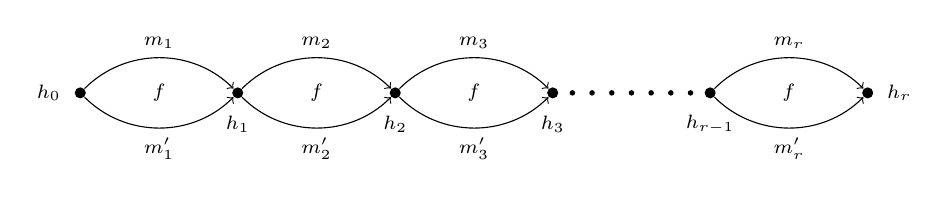
\begin{tikzpicture}[scale=1]
        
           \draw (0,0) node[fill,circle,inner sep=0pt,minimum size=4pt] (a1) {};%
           \draw (2,0) node[fill,circle,inner sep=0pt,minimum size=4pt] (a2) {};%
           \draw (4,0) node[fill,circle,inner sep=0pt,minimum size=4pt] (a3) {};%
           \draw (6,0) node[fill,circle,inner sep=0pt,minimum size=4pt] (a4) {};%
        
           \draw (6.25,0) node[fill,circle,inner sep=0pt,minimum size=2pt] (b0) {};%
           \draw (6.5,0) node[fill,circle,inner sep=0pt,minimum size=2pt] (b1) {};%
           \draw (6.75,0) node[fill,circle,inner sep=0pt,minimum size=2pt] (b2) {};%
           \draw (7,0) node[fill,circle,inner sep=0pt,minimum size=2pt] (b3) {};%
           \draw (7.25,0) node[fill,circle,inner sep=0pt,minimum size=2pt] (b4) {};%
           \draw (7.5,0) node[fill,circle,inner sep=0pt,minimum size=2pt] (b5) {};%
           \draw (7.75,0) node[fill,circle,inner sep=0pt,minimum size=2pt] (b6) {};%
        
           \draw (8,0) node[fill,circle,inner sep=0pt,minimum size=4pt] (a5) {};%
           \draw (10,0) node[fill,circle,inner sep=0pt,minimum size=4pt] (a6) {};%
          
           \draw[->] (a1) edge[out= 45, in= 3*45] node[above]{\scriptsize $m_{1}$} (a2);
           \draw[->] (a1) edge[out=-45, in=-3*45] node[below]{\scriptsize $m'_{1}$} (a2);
          
           \draw[->] (a2) edge[out= 45, in= 3*45] node[above]{\scriptsize $m_{2}$} (a3);
           \draw[->] (a2) edge[out=-45, in=-3*45] node[below]{\scriptsize $m'_{2}$} (a3);
          
           \draw[->] (a3) edge[out= 45, in= 3*45] node[above]{\scriptsize $m_{3}$} (a4);
           \draw[->] (a3) edge[out=-45, in=-3*45] node[below]{\scriptsize $m'_{3}$} (a4);
           
           \draw[->] (a5) edge[out= 45, in= 3*45] node[above]{\scriptsize $m_{r}$} (a6);
           \draw[->] (a5) edge[out=-45, in=-3*45] node[below]{\scriptsize $m'_{r}$} (a6);
           
           \path (1,0) node {\scriptsize $f$};
           \path (3,0) node {\scriptsize $f$};
           \path (5,0) node {\scriptsize $f$};
           \path (9,0) node {\scriptsize $f$};
           
          
           \path (-0.4,0) node {\scriptsize $h_{0}$};
           \path (2,-0.4) node {\scriptsize $h_{1}$};
           \path (4,-0.4) node {\scriptsize $h_{2}$};
           \path (6,-0.4) node {\scriptsize $h_{3}$};
           \path (8,-0.4) node {\scriptsize $h_{r-1}$};
           \path (10+0.4,0) node {\scriptsize $h_{r}$};
        
        \end{tikzpicture}
    }
    \begin{outline}
        \1 $2^{r}$ collisions sur $h_r$ générées pour le prix de $r$
        \pause
        \1 Dans notre cas
            \2 On génère facilement $2^{24}$ collisions $md5(x_1)= \cdots = md5(x_{2^{24}})$
            \pause
            \2 On itère sur $2^{24}$ valeurs de $a$ jusqu'à avoir la collision sur $md5(x_1 || a)$
            \pause
            \2 Statistiquement, il y a une collision pour au moins un des $sha1(x_i || a)$  $\flag$
    \end{outline}
\end{frame}
